% ============================================================================
\section{Multimodality}
% ============================================================================

\begin{frame}[t]{Vision--Language Models: naming and motivation (Recap)}
  \begin{itemize}\itemsep0.4em
    \item As covered earlier, pairing vision with language lets a user specify a new task in words (``what species of bird is this?'', ``read the sign in the corner'') instead of collecting a fresh label set for every concept.
    \item Nomenclature (informal): an \textbf{LLM} is language-first; a \textbf{VLM} adds a vision encoder so the stack can condition on images; an \textbf{MLLM} usually means several modalities (image, video, audio) in one family.
    \item The architectural question this section answers is narrower: at what point in the stack do image tokens meet the language model, and what does each answer cost?
  \end{itemize}
  \vfill
  {\scriptsize Bandaru, \textit{Vision Language Models} (blog, Aug.\ 2025), \href{https://rohitbandaru.github.io/blog/Vision-Language-Models/}{rohitbandaru.github.io/blog/Vision-Language-Models/}.}
\end{frame}

\begin{frame}[t]{Fusion Patterns: Where do image tokens meet the LLM?}
  \begin{itemize}
    \item Early fusion: build one long token sequence (visual tokens + text tokens) and run attention over the mixture. This is what most ``native'' VLMs aim for today.
    \item Middle fusion: insert vision cross-attention inside some transformer blocks. This is the usual choice when retrofitting vision onto a stack that was already trained on text alone.
    \item Late fusion: encode each modality separately and compare the two embeddings at the end. Right for retrieval and zero-shot scoring, as in CLIP, but too weak for open-ended captioning or VQA, because the language model never receives rich visual state.
    \item Images create many tokens; good designs compress visual length (pooling, grouping, tiling) before the LLM sees them.
  \end{itemize}
\end{frame}

\begin{frame}[t]{Early fusion: linear or MLP projector}
  \begin{itemize}
    \item Freeze (or lightly train) a strong ViT; map its patch tokens through a small projector into the LLM embedding width, then concatenate with text tokens.
    \item Simple, stable, and very common in open recipes. The projector is a single linear map in LLaVA~v1 and PaliGemma~2, and a two-layer MLP in LLaVA-1.5, DeepSeek-VL, and LLaMA~4.
  \end{itemize}
  \centering
  
\includegraphics[width=0.92\textwidth,height=0.46\textheight,keepaspectratio]{images/transformers-2017-v-2026/bandaru_vlm_llava_architecture.png}\\[0.15em]
  {\scriptsize Liu et al., LLaVA, \href{https://arxiv.org/abs/2304.08485}{arXiv:2304.08485}, Figure~1; via Bandaru, \textit{Vision Language Models} (blog).}
\end{frame}

\begin{frame}[t]{Early fusion: cross-attention adapter}
  \begin{itemize}
    \item A small adapter uses learned query vectors that cross-attend to the ViT tokens and emit a fixed, short set of visual summaries (256 in Qwen-VL) that are then concatenated with the text tokens.
    \item The cross-attention lives in the adapter, outside the language model, so the LLM stack is unchanged and still sees one mixed sequence. That is what keeps this early rather than middle fusion.
  \end{itemize}
  \centering
  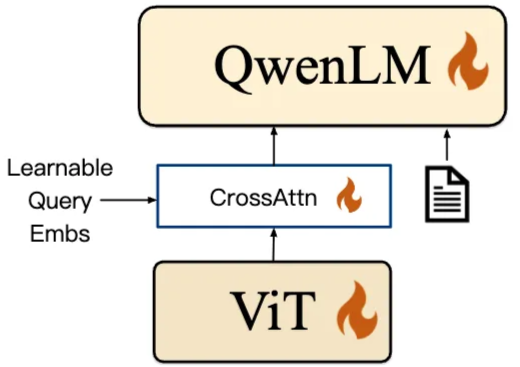
\includegraphics[width=\textwidth,height=0.40\textheight,keepaspectratio]{images/transformers-2017-v-2026/bandaru_vlm_qwen_vl_adapter.png}
  \vfill
  {\scriptsize Bai et al., Qwen-VL, \href{https://arxiv.org/abs/2308.12966}{arXiv:2308.12966}, Figure~3 (multi-task pre-training stage); via Bandaru, \textit{Vision Language Models} (blog).}
\end{frame}

\begin{frame}[t]{Middle fusion: Flamingo}
  \begin{itemize}
    \item Keep the pretrained vision encoder and LLM frozen; insert Perceiver resamplers (compress a variable number of vision features to a fixed 64 tokens) and gated cross-attention blocks inside the LLM stack.
    \item The vision encoder here is an NFNet-F6, not a ViT: Flamingo predates the convention of pairing every LLM with a vision transformer.
  \end{itemize}
  \centering
  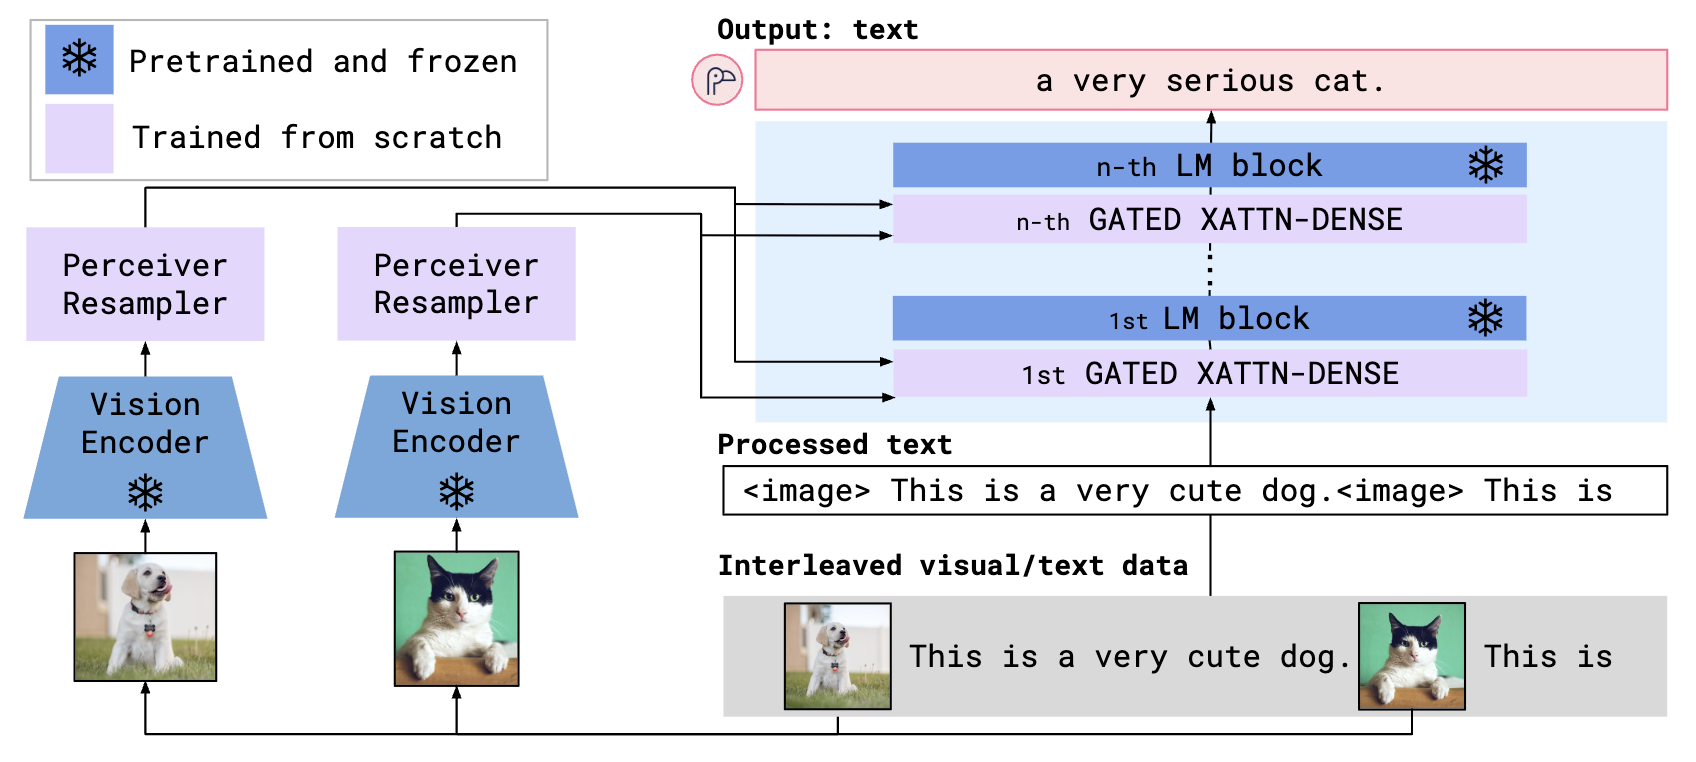
\includegraphics[width=\textwidth,height=0.50\textheight,keepaspectratio]{images/transformers-2017-v-2026/bandaru_vlm_flamingo_architecture.png}
  \vfill
  {\scriptsize Alayrac et al., Flamingo, \href{https://arxiv.org/abs/2204.14198}{arXiv:2204.14198}, Figure~3; via Bandaru, \textit{Vision Language Models} (blog).}
\end{frame}

\begin{frame}[t]{Middle fusion: LLaMA 3}
  \begin{itemize}\itemsep0.4em
    \item \textbf{ViT encoder:} ViT-H/14 (630M parameters, 32 blocks) trained CLIP-style for image--text alignment; features are taken from several intermediate layers, not only the last.
    \item \textbf{Decoder:} a cross-attention layer after every fourth self-attention layer, tanh-gated with the gates initialized to zero so the vision path starts as a no-op and is learned in. The language weights are never updated.
    \item \textbf{Why middle fusion:} it suits LLaMA 3's text-first design, since vision is added to a finished language model. LLaMA 4 moves to early fusion so that text and image tokens can be trained together from the start.
  \end{itemize}
  \vfill
  {\scriptsize Grattafiori et al., ``The Llama 3 Herd of Models,'' \href{https://arxiv.org/abs/2407.21783}{arXiv:2407.21783}, Sec.~7.}
\end{frame}
